\documentclass[tikz, margin=3.14mm]{standalone}

\usepackage{tikz}
\usetikzlibrary{decorations, calc, arrows, arrows.meta, positioning}

\begin{document}
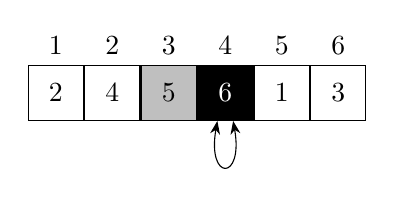
\begin{tikzpicture}[
    >=Stealth,
    array/.style={rectangle, draw, inner sep=5pt, text=black,
        minimum width = 20pt, minimum height = 20pt}
]

    % Nodes ------------------------------------------------------

    \node[array] (n1) {2};
    \node[array, right=0cm of n1] (n2) {4};
    \node[array, right=0cm of n2, fill = lightgray] (n3) {5};
    \node[array, right=0cm of n3, fill = black, text = white] (n4) {6};
    \node[array, right=0cm of n4] (n5) {1};
    \node[array, right=0cm of n5] (n6) {3};

    % labels
    \node[above=0cm of n1] (n1_label) {1};
    \node[above=0cm of n2] (n2_label) {2};
    \node[above=0cm of n3] (n3_label) {3};
    \node[above=0cm of n4] (n4_label) {4};
    \node[above=0cm of n5] (n5_label) {5};
    \node[above=0cm of n6] (n6_label) {6};

    % Arrows ---------------------------------------------------

    \draw [<->] ($(n4.south)-(.1,0)$) to[out=-100, in=-80, looseness=10] ($(n4.south)+(.1,0)$);

\end{tikzpicture}
\end{document}